\section{Aufbau der NE555 Timerschaltung}
Ziel dieser Aufgabe ist es mithilfe eines NE555-Timers ein Rechteckssignal für die weitere Schaltung zu erzeugen.

\subsection{Schaltung}
Die Schaltung \cref{fig:schaltung_ne555} besteht aus einem NE555 Timer-Baustein.

\begin{figure}[h]
  \centering
  \caption{Schaltung der Timerschaltung}
  \label{fig:schaltung_ne555}
\end{figure}

\subsection{Messvorgang}
Es wurde das Ausgangssignal $U_{PWM}$ der Schaltung mithilfe des Oszilloskops gemessen und die Frequenz mit Hilfe des Potentiometers an die gewünschten 130kHz angeglichen.

\subsection{Messergebnis}
\begin{figure}[H]
  \centering
  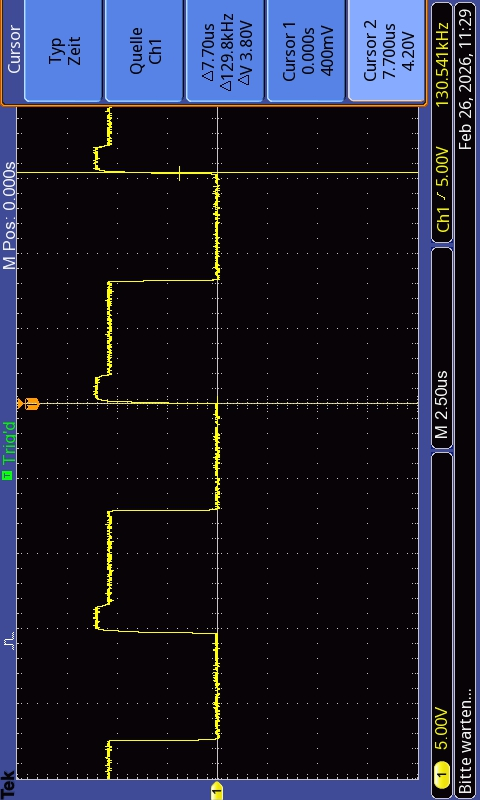
\includegraphics[width=0.4\linewidth, angle=-90]{Timerschaltung/NE555_Output_kalibriert}
  \caption{$U_{PWM}$ der Timerschaltung}
  \label{fig:ne555outputkalibriert}
\end{figure}

\subsection{Interpretation}
In der \cref{fig:ne555outputkalibriert} ist zu erkennen dass eine Periode von $U_{PWM}\approx 130\, kHz$ erreicht wird.
